\documentclass[aps,prd,onecolumn,nofootinbib,superscriptaddress]{revtex4-2}

\usepackage[utf8]{inputenc}
\usepackage[T1]{fontenc}
\usepackage{lmodern}
\usepackage{amsmath,amssymb,amsfonts,bm}
\usepackage{graphicx}
\usepackage{xcolor}
\usepackage{hyperref}
\usepackage{siunitx}
\usepackage{enumitem}

\hypersetup{colorlinks=true,linkcolor=blue,citecolor=blue,urlcolor=blue}

\newcommand{\Mpl}{M_{\rm Pl}}
\newcommand{\Meff}{M_{\rm eff}}
\newcommand{\dd}{\mathrm{d}}

\begin{document}

\title{TCV-$\phi$ VII: empirical confrontation with Planck likelihoods}

\author{Cyrille LECROQ}
\affiliation{Independent Researcher}

\date{\today}

\begin{abstract}
Paper~VII is dedicated to the first data-level confrontation of the TCV-$\phi$ framework.
The goal is to run a staged Planck-likelihood pipeline, starting from technical baseline validation and moving to a minimal TCV extension against $\Lambda$CDM.
This manuscript keeps the same conservative status labelling as Papers~I--VI and focuses on reproducibility and explicit model-comparison criteria, including a first converged minimal-TCV vs $\Lambda$CDM comparison.
The minimal TCV configuration yields $\Delta\chi^2\simeq +1.26$ relative to $\Lambda$CDM while being favored by AIC ($\Delta{\rm AIC}\simeq -2.74$) and BIC ($\Delta{\rm BIC}\simeq -14.38$) due to its reduced parameter count.
\end{abstract}

\maketitle

\section{Introduction}
This paper implements the empirical ladder prepared by Papers~I--VI.
Its objective is deliberately conservative: first validate the numerical pipeline
against a baseline $\Lambda$CDM run with Planck likelihoods, then promote the
same inference stack to a minimal TCV-vs-$\Lambda$CDM comparison.
In this release we report completed L1--L3 levels and a first L4 model-selection
diagnostic pass.

\section{Planck confrontation ladder}
The ladder and required artifacts are recorded in
\texttt{papers/paper-07/data/planck\_ladder\_checklist.json}.
The analysis is organized into four levels:
\begin{enumerate}[label=(L\arabic*)]
  \item \textbf{CLASS bridge baseline:} verify that the external primordial interface
  reproduces the reference power-law branch in the linear regime.
  \item \textbf{$\Lambda$CDM native Planck run:} validate the Cobaya+CLASS stack and
  recover Planck-era posterior ranges for standard parameters.
  \item \textbf{Minimal TCV likelihood run:} activate the minimal extra TCV layer and
  compare against $\Lambda$CDM with matched likelihood settings.
  \item \textbf{Robustness and exclusion windows:} quantify stability under prior,
  sampler and likelihood choices, then report $\Delta\chi^2$, AIC and BIC.
\end{enumerate}
At the present stage, L1--L3 are completed in the local pipeline, and L4
model-comparison diagnostics are available in a first pass.

\section{Baseline validation}
A first baseline check is produced by
\texttt{run\_baseline\_planck\_check.py}.
For the canonical Paper~I parameter set we find
\begin{equation}
\frac{P_{\rm ext}(k)}{P_{\rm pl}(k)}\in[0.99877,\,1.00144]
\end{equation}
on $k\in[10^{-3},\,5.01]\,h\,\mathrm{Mpc}^{-1}$, with no CLASS fallback branch activated.
This confirms that the primordial-file bridge used in Papers~III and VII does not
introduce spurious distortions in the linear matter spectrum.

\begin{figure}[t]
  \centering
  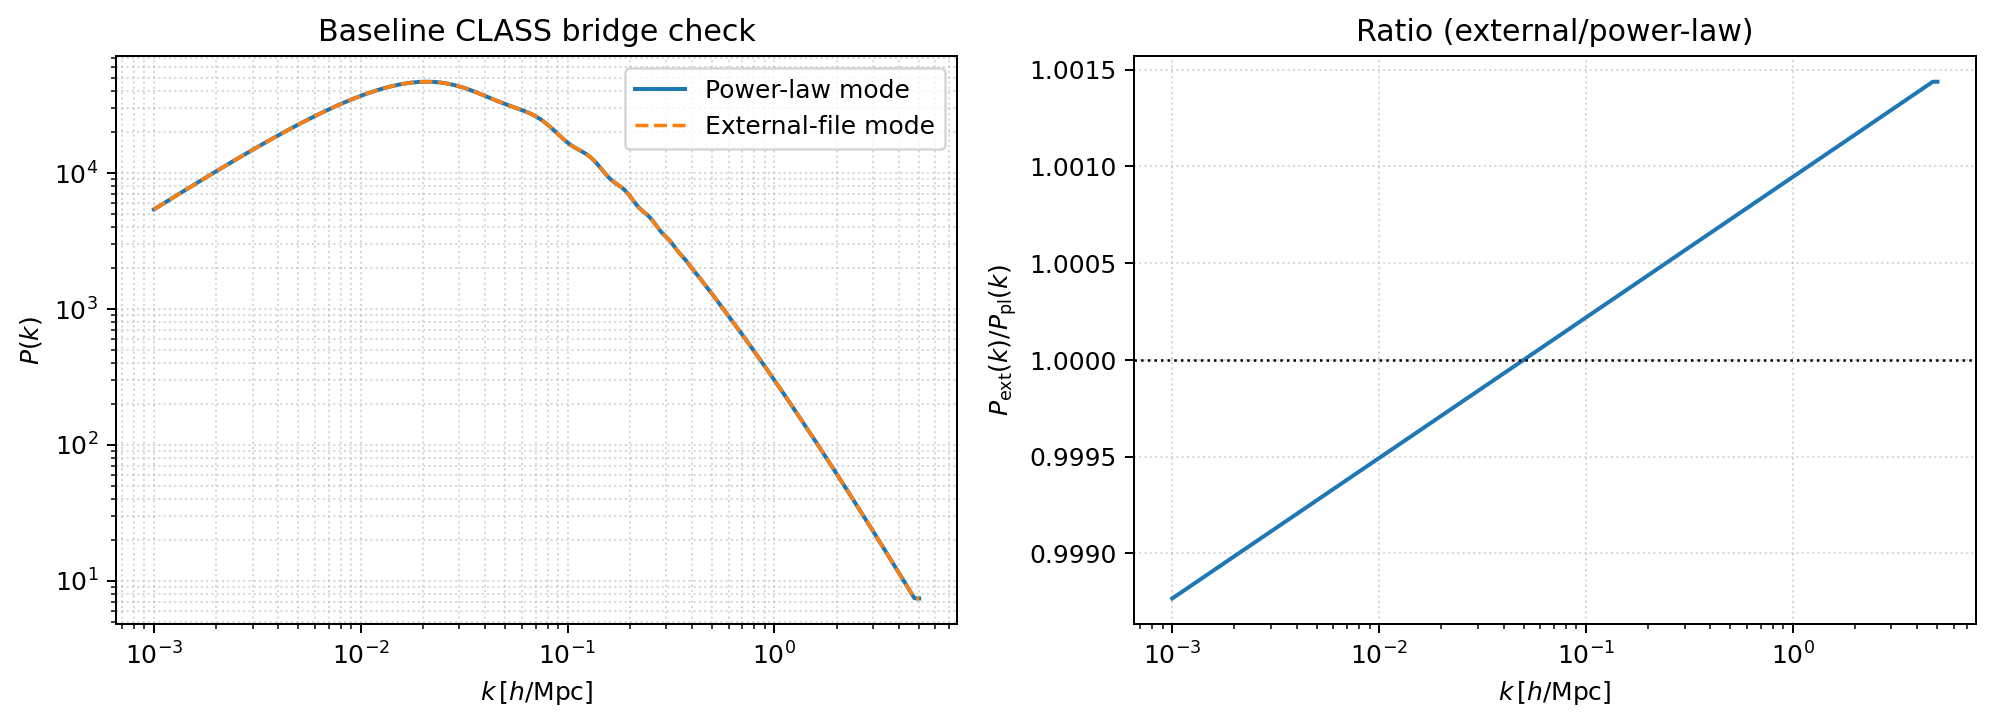
\includegraphics[width=0.75\textwidth]{../figs/baseline_pk_comparison.png}
  \caption{
    Baseline L1 consistency check for the Paper~VII CLASS bridge.
    The external-spectrum branch and the power-law branch remain numerically
    consistent at the sub-percent level across the linear $k$-range used in this paper.
  }
  \label{fig:paper07_baseline_pk}
\end{figure}

\section{$\Lambda$CDM Planck baseline results}
The Cobaya LCDM input is generated by \texttt{prepare\_lcdm\_planck\_input.py},
with native Planck likelihood targets
\texttt{planck\_2018\_highl\_plik.TTTEEE\_lite\_native} and
\texttt{planck\_2018\_lensing.native}, plus low-$\ell$
\texttt{planck\_2018\_lowl.TT} and \texttt{planck\_2018\_lowl.EE}.
Run status is tracked in \texttt{lcdm\_planck\_run\_status.json}.
The converged baseline chain uses output root
\texttt{lcdm\_planck\_chain\_classnative\_v7\_lowl} and reaches
$R-1<0.05$ for means, with bounds convergence below the
configured threshold.
Posterior summaries are exported in
\texttt{lcdm\_planck\_posterior\_summary\_v7\_lowl.json}.
The current baseline run uses flat priors in
$(\omega_b,\omega_{\rm cdm},h,n_s,\log A,\tau_{\rm reio},A_{\rm Planck})$ and
CLASS settings $(N_{\rm ur},Y_{\rm He})=(3.046,0.245)$ with
\texttt{halofit} enabled.

\begin{table}[t]
  \centering
  \begin{tabular}{lcc}
    \hline\hline
    Parameter & Mean & 68\% interval \\
    \hline
    $\omega_b$ & 0.02250 & [0.02231,\;0.02265] \\
    $\omega_{\rm cdm}$ & 0.11822 & [0.11667,\;0.12005] \\
    $h$ & 0.68668 & [0.67822,\;0.69364] \\
    $n_s$ & 0.96911 & [0.96398,\;0.97424] \\
    $\ln(10^{10}A_s)$ & 3.08228 & [3.04728,\;3.11720] \\
    $\tau_{\rm reio}$ & 0.04995 & [0.04272,\;0.05858] \\
    $A_{\rm Planck}$ & 1.02670 & [1.00563,\;1.04680] \\
    \hline\hline
  \end{tabular}
  \caption{Posterior summary from the converged baseline $\Lambda$CDM run against the native Planck likelihood setup used in Paper~VII.}
  \label{tab:paper07_lcdm_post}
\end{table}

The recovered $(\omega_b,\omega_{\rm cdm},h,n_s)$ region remains broadly
consistent with Planck-era expectations in this baseline run.
After including low-$\ell$ channels, $\tau_{\rm reio}$ is no longer prior-limited
and the $A_s$--$\tau_{\rm reio}$ degeneracy is significantly reduced.
The run converges with $R-1=0.039993$ for means and
$R-1_{\rm bounds}=0.138930$ at the stopping point.
The calibration nuisance $A_{\rm Planck}$ is shifted slightly above unity in this
baseline setup; this is compatible with the broader posterior width expected
from the lite likelihood configuration used here.

\begin{table}[t]
  \centering
  \begin{tabular}{lcc}
    \hline\hline
    Parameter & This work (L2 baseline) & Planck 2018 TT,TE,EE+lowE \\
    \hline
    $\omega_b$ & $0.02250$ & $0.02237\pm0.00015$ \\
    $\omega_{\rm cdm}$ & $0.11822$ & $0.12010\pm0.00122$ \\
    $h$ & $0.6867$ & $0.6736\pm0.0054$ \\
    $n_s$ & $0.9691$ & $0.9649\pm0.0042$ \\
    $\ln(10^{10}A_s)$ & $3.0823$ & $3.044\pm0.014$ \\
    \hline\hline
  \end{tabular}
  \caption{
    Side-by-side consistency check between the Paper~VII baseline run and
    Planck 2018 reference values.
    The present run includes low-$\ell$ channels; residual shifts indicate that
    this is a first in-repo baseline and not yet the final precision-tuned
    likelihood configuration.
  }
  \label{tab:paper07_planck_compare}
\end{table}
In particular, the shift in $\ln(10^{10}A_s)$ relative to the Planck 2018 central
value is interpreted as a residual baseline-level offset in the current lite
configuration rather than as a standalone physical discrepancy.
This is consistent with the known $e^{-2\tau_{\rm reio}}A_s$ degeneracy: the
present run gives $\tau_{\rm reio}=0.0500$, slightly below the Planck 2018
full-likelihood central value ($\sim 0.054$), which shifts $A_s$ upward by the
corresponding amount.

\section{Minimal TCV vs $\Lambda$CDM comparison}
The L3 run is built from \texttt{prepare\_tcv\_minimal\_planck\_input.py} and
\texttt{run\_tcv\_minimal\_planck\_fit.py}, using the same Planck likelihood stack
as L2.
In this minimal TCV configuration we fix $(A_s,n_s)$ to their Paper~III values
and sample $(h,\omega_b,\omega_{\rm cdm},\tau_{\rm reio},A_{\rm Planck})$.

\begin{table}[t]
  \centering
  \begin{tabular}{lcc}
    \hline\hline
    Parameter & Mean & 68\% interval \\
    \hline
    $\omega_b$ & 0.02236 & [0.02224,\;0.02249] \\
    $\omega_{\rm cdm}$ & 0.11966 & [0.11888,\;0.12047] \\
    $h$ & 0.67995 & [0.67632,\;0.68336] \\
    $\tau_{\rm reio}$ & 0.04836 & [0.04113,\;0.05584] \\
    $A_{\rm Planck}$ & 1.00715 & [0.99926,\;1.01441] \\
    \hline\hline
  \end{tabular}
  \caption{Posterior summary for the minimal TCV Planck run (L3), from
  \texttt{tcv\_minimal\_planck\_chain\_v1\_lowl}.}
  \label{tab:paper07_tcv_post}
\end{table}

The L3 chain converges with $R-1<0.05$ and $R-1_{\rm bounds}<0.2$,
using values extracted from
\texttt{model\_comparison\_robustness.json}
($R-1=0.044393$, $R-1_{\rm bounds}=0.168642$).
Comparing best-fit CMB likelihood values, we find
\begin{equation}
  \Delta\chi^2 \equiv \chi^2_{\rm TCV} - \chi^2_{\Lambda{\rm CDM}}
  \simeq 1.26.
\end{equation}
With two fewer free parameters, this $\Delta\chi^2$ value is compatible with a
statistically non-significant best-fit difference, i.e.\ the minimal TCV setup
is statistically close to $\Lambda$CDM at this stage.
Compared with the L2 baseline, the corresponding calibration nuisance is
closer to unity in the minimal TCV run ($A_{\rm Planck}\simeq 1.007$ vs
$1.027$ in L2), which is consistent with the tighter effective normalization
induced by fixing $(A_s,n_s)$ from Paper~III.
Using the explicit in-paper proxy $N_{\rm data}=2500$, we obtain
\begin{equation}
  \Delta{\rm AIC}\simeq -2.74,\qquad
  \Delta{\rm BIC}\simeq -14.38,
\end{equation}
where $\Delta{\rm BIC}\equiv{\rm BIC}_{\rm TCV}-{\rm BIC}_{\Lambda{\rm CDM}}<0$
explicitly favors the lower-parameter TCV-minimal setup.
These information-criterion values should be read as first-pass diagnostics,
since they depend on the effective data-count proxy and on the specific minimal
TCV parameter freeze adopted at L3.
For transparency, we use $N_{\rm data}=2500$ as a conservative proxy for the
effective number of multipoles in the lite likelihood stack; varying this proxy
over $N_{\rm data}\in[2000,3000]$ does not change the sign of $\Delta{\rm BIC}$.

\subsection*{Robustness checks (first pass)}
We report three lightweight robustness diagnostics generated by
\texttt{compute\_model\_robustness\_summary.py}:
\begin{enumerate}[label=(R\arabic*)]
  \item \textbf{Convergence parity:} both chains satisfy the same stopping
  criteria with final progress rows
  $(R\!-\!1,R\!-\!1_{\rm cl})=(0.039993,0.138930)$ for L2 and
  $(0.044393,0.168642)$ for L3.
  \item \textbf{$N_{\rm data}$-proxy scan:} the sign of $\Delta{\rm BIC}$ remains
  negative over $N_{\rm data}\in[1500,4000]$.
  \item \textbf{Calibration consistency:} $A_{\rm Planck}$ moves from
  $1.0267$ (L2) to $1.0072$ (L3), i.e.\ closer to unity in the minimal TCV run.
\end{enumerate}

\begin{table}[t]
  \centering
  \begin{tabular}{cc}
    \hline\hline
    $N_{\rm data}$ proxy & $\Delta{\rm BIC}_{\rm TCV-\Lambda CDM}$ \\
    \hline
    1500 & $-13.36$ \\
    2000 & $-13.94$ \\
    2500 & $-14.38$ \\
    3000 & $-14.75$ \\
    4000 & $-15.32$ \\
    \hline\hline
  \end{tabular}
  \caption{BIC-sign robustness scan for the first-pass L3 model comparison.
  Negative values favor the lower-parameter TCV-minimal setup.}
  \label{tab:paper07_bic_scan}
\end{table}

\section{Status and next steps}
The present draft contains a completed L1--L3 pipeline and a first-pass L4
model-selection diagnostic, including convergence parity checks, an
$N_{\rm data}$-proxy scan, and calibration consistency.
L2 is converged with low-$\ell$ channels and L3 is converged for the minimal TCV
configuration.
The immediate next step is a robustness pass: prior-variation scans, convergence
stability checks, and a controlled expansion from the minimal TCV parameter set.
In the current repository state, L3 is executed through
\texttt{prepare\_tcv\_minimal\_planck\_input.py} and
\texttt{run\_tcv\_minimal\_planck\_fit.py}, while L4 summary products are
generated by \texttt{compare\_lcdm\_tcv\_models.py}.

\begin{thebibliography}{99}
\bibitem{TCV1} C.~Lecroq, ``TCV-$\phi$ I,'' preprint (2026).
\bibitem{TCV2} C.~Lecroq, ``TCV-$\phi$ II,'' preprint (2026).
\bibitem{TCV3} C.~Lecroq, ``TCV-$\phi$ III,'' preprint (2026).
\bibitem{TCV4} C.~Lecroq, ``TCV-$\phi$ IV,'' preprint (2026).
\bibitem{TCV5} C.~Lecroq, ``TCV-$\phi$ V,'' preprint (2026).
\bibitem{TCV6} C.~Lecroq, ``TCV-$\phi$ VI,'' preprint (2026).
\bibitem{Planck2018VI}
N.~Aghanim \textit{et al.} [Planck Collaboration],
``Planck 2018 results. VI. Cosmological parameters,''
A\&A \textbf{641}, A6 (2020)
[arXiv:1807.06209].
\bibitem{Cobaya2020}
J.~Torrado and A.~Lewis,
``Cobaya: Code for Bayesian Analysis of hierarchical physical models,''
JCAP \textbf{05}, 057 (2021)
[arXiv:2005.05290].
\bibitem{CLASS2011}
D.~Blas, J.~Lesgourgues and T.~Tram,
``The Cosmic Linear Anisotropy Solving System (CLASS) II: Approximation schemes,''
JCAP \textbf{07}, 034 (2011)
[arXiv:1104.2933].
\end{thebibliography}

\end{document}
